\section{Nodes}

A node is a Linux machine with special software installed, called ORC, which enables OCTA CORE to establish a secure communication channel with the node.

The communication between \textbf{OCTA CORE} and \textbf{ORC} is done in an RPC\cite{rpc}-like manner,
and a secure channel is implemented using the HTTPS\cite{https} protocol, with each request being validated using a security token.

\begin{figure}[H]
    \centering
    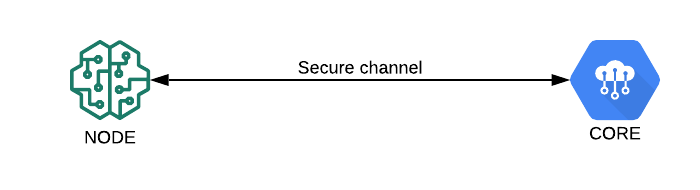
\includegraphics[scale=0.5]{core-orc-channel}
    \caption{Secure communication channel}
\end{figure}

\textbf{ORC} is responsible for the following activities:

\begin{itemize}
    \item Detecting installed hardware suchas CPU, GPUs, RAM, volume of disk storage
    \item Collecting metrics about hardware usage, suhc as free/used disk/ram space, CPU and GPU load, temperature and fans speed
    \item Manage Docker\cite{docker} containers and Firecracker\cite{firecracker} microVMs
\end{itemize}

There are two types of nodes: \textbf{blockchain} and \textbf{service}

The blockchain node supports the OCTA Layer 1 blockchain by running network node software, which makes the network more stable, distributed, more latency fair, and speeds up synchronization.

The service node provides resources that are used to implement services for end-users.

\subsection{Hardware and software requirements}

To cover a wide range of supported hardware, node software can be installed on any machine with x86\_64\cite{x86_64} or ARM\cite{arm} architecture.

In order to run the node, the hardware must meet the minimum system requirements, which are as follows: 1 CPU, 1 Gb of RAM, and 10Gb of free disk space.

However, the requirements for hardware may vary depending on the intended purpose of the node. For instance, a node that provides only VPN services may only need to meet the minimum requirements. Conversely, nodes that are designed to perform AI/ML tasks will require powerful GPUs connected with a high bandwidth PCIe interface, as well as ample disk storage.

It's worth noting that both NVIDIA and AMD GPUs are supported by the system.

To determine the performance of a node, the following measurements are taken:

\begin{itemize}
    \item Network upload/download speed
    \item Disk write speed
    \item GPU performance using AI benchmark (only for NVIDIA)
\end{itemize}

These performance metrics help users to choose the hardware they need for their tasks.

The node software can be installed on any Linux distribution; however, we primarily focus on Ubuntu LTS or Debian as the recommended operating systems.

Windows Subsystem for Linux (WSL) has limited support.

\subsection{Security}

Security is of utmost importance to us, and we take various measures to eliminate possible security risks for users running our software ORC on their machines.

We follow a set of rules and guidelines to ensure the security of our system, which includes:

\begin{itemize}
    \item Open-sourcing \textbf{ORC}, which allows for audits by other people to ensure that the software does not have any malicious code
    \item Keeping code base of \textbf{ORC} as small as possible for ease of auditing
    \item Running node software under a non-privileged user and not granting any permissions that are not needed for its operation
    \item Regular software updates to ensure that the latest security patches are applied. Along with comprehensive testing of software to detect and address any potential security issues
\end{itemize}

These measures are in place to ensure that our users can have peace of mind when using our system, and their data and resources are secure.

We take the security of our users very seriously and are continuously working to improve our system's security features.

\subsection{Verification}

Verification is critical to ensuring that the node infrastructure operates smoothly and reliably, which is essential for providing high-quality services to end-users.
Every new node that joins the OctaSpace cloud must be verified and confirmed to meet the necessary requirements to provide services.

Periodic re-verification checks are conducted on verified nodes. It is therefore essential to monitor the status of your nodes to avoid them being changed to an unverified status.

The checks performed to ensure that the node is properly configured may include, but are not limited to:

\begin{itemize}
    \item Meeting minimum hardware requirements
    \item Synchronized system clock
    \item All necessary network ports are open
    \item Correct installation of the GPU driver
\end{itemize}

The list of checks will be expanding in the future to ensure even greater accuracy and reliability.

The following restrictions are applied for the unverified nodes:

\begin{itemize}
    \item Unable to provide services
    \item Unable to participate in staking \hyperref[sec:staking]{staking}
\end{itemize}
